\textit{written by L.B. and B.L.}\\

The frontend has been developed in Streamlit \cite{streamlit2018} in its latest version as of \today, 0.82.0, and can be accessed at \url{https://clustering.goethe.tech)}.
On the left there is a sidebar containing two collapsible content groups. One of them is called \mintinline[bgcolor=code-bg]{python}{Regular} and comprises controls for a single clustering method. The other one named \mintinline[bgcolor=code-bg]{python}{Comparison} contains controls for a workflow that lets the user compare the different methods.
First off, there is the \mintinline[bgcolor=code-bg]{python}{Regular} group. It provides a menu containing two dropdown lists. While the upper dropdown list can be used to select the data set to be clustered, the second dropdown contains four different clustering algorithms to be applied: K-Means, Mean Shift, Spectral Clustering and Affinity Propagation. According to the selected clustering algorithm, the required input parameter can be set by dragging the slider on the respective widget. For this purpose, a message displays which kind of input parameter is required for the selected algorithm. 
Default values for different parameters vary with regard to the chosen data set. We therefore provide slider widgets with different value ranges and varying default values according to the data set to be clustered.
Once data set and clustering technique are chosen, the \mintinline[bgcolor=code-bg]{python}{Calculate} button can be clicked to run the clustering procedure.
%For convenience, selected dataset and algorithms are listed above the result part once again. 
After the dataset is clustered, a two-dimensional projection plot of all data points is displayed within the main panel, distinguishing between different clusters with the help of distinct symbols and colors.

\begin{figure}[H]
%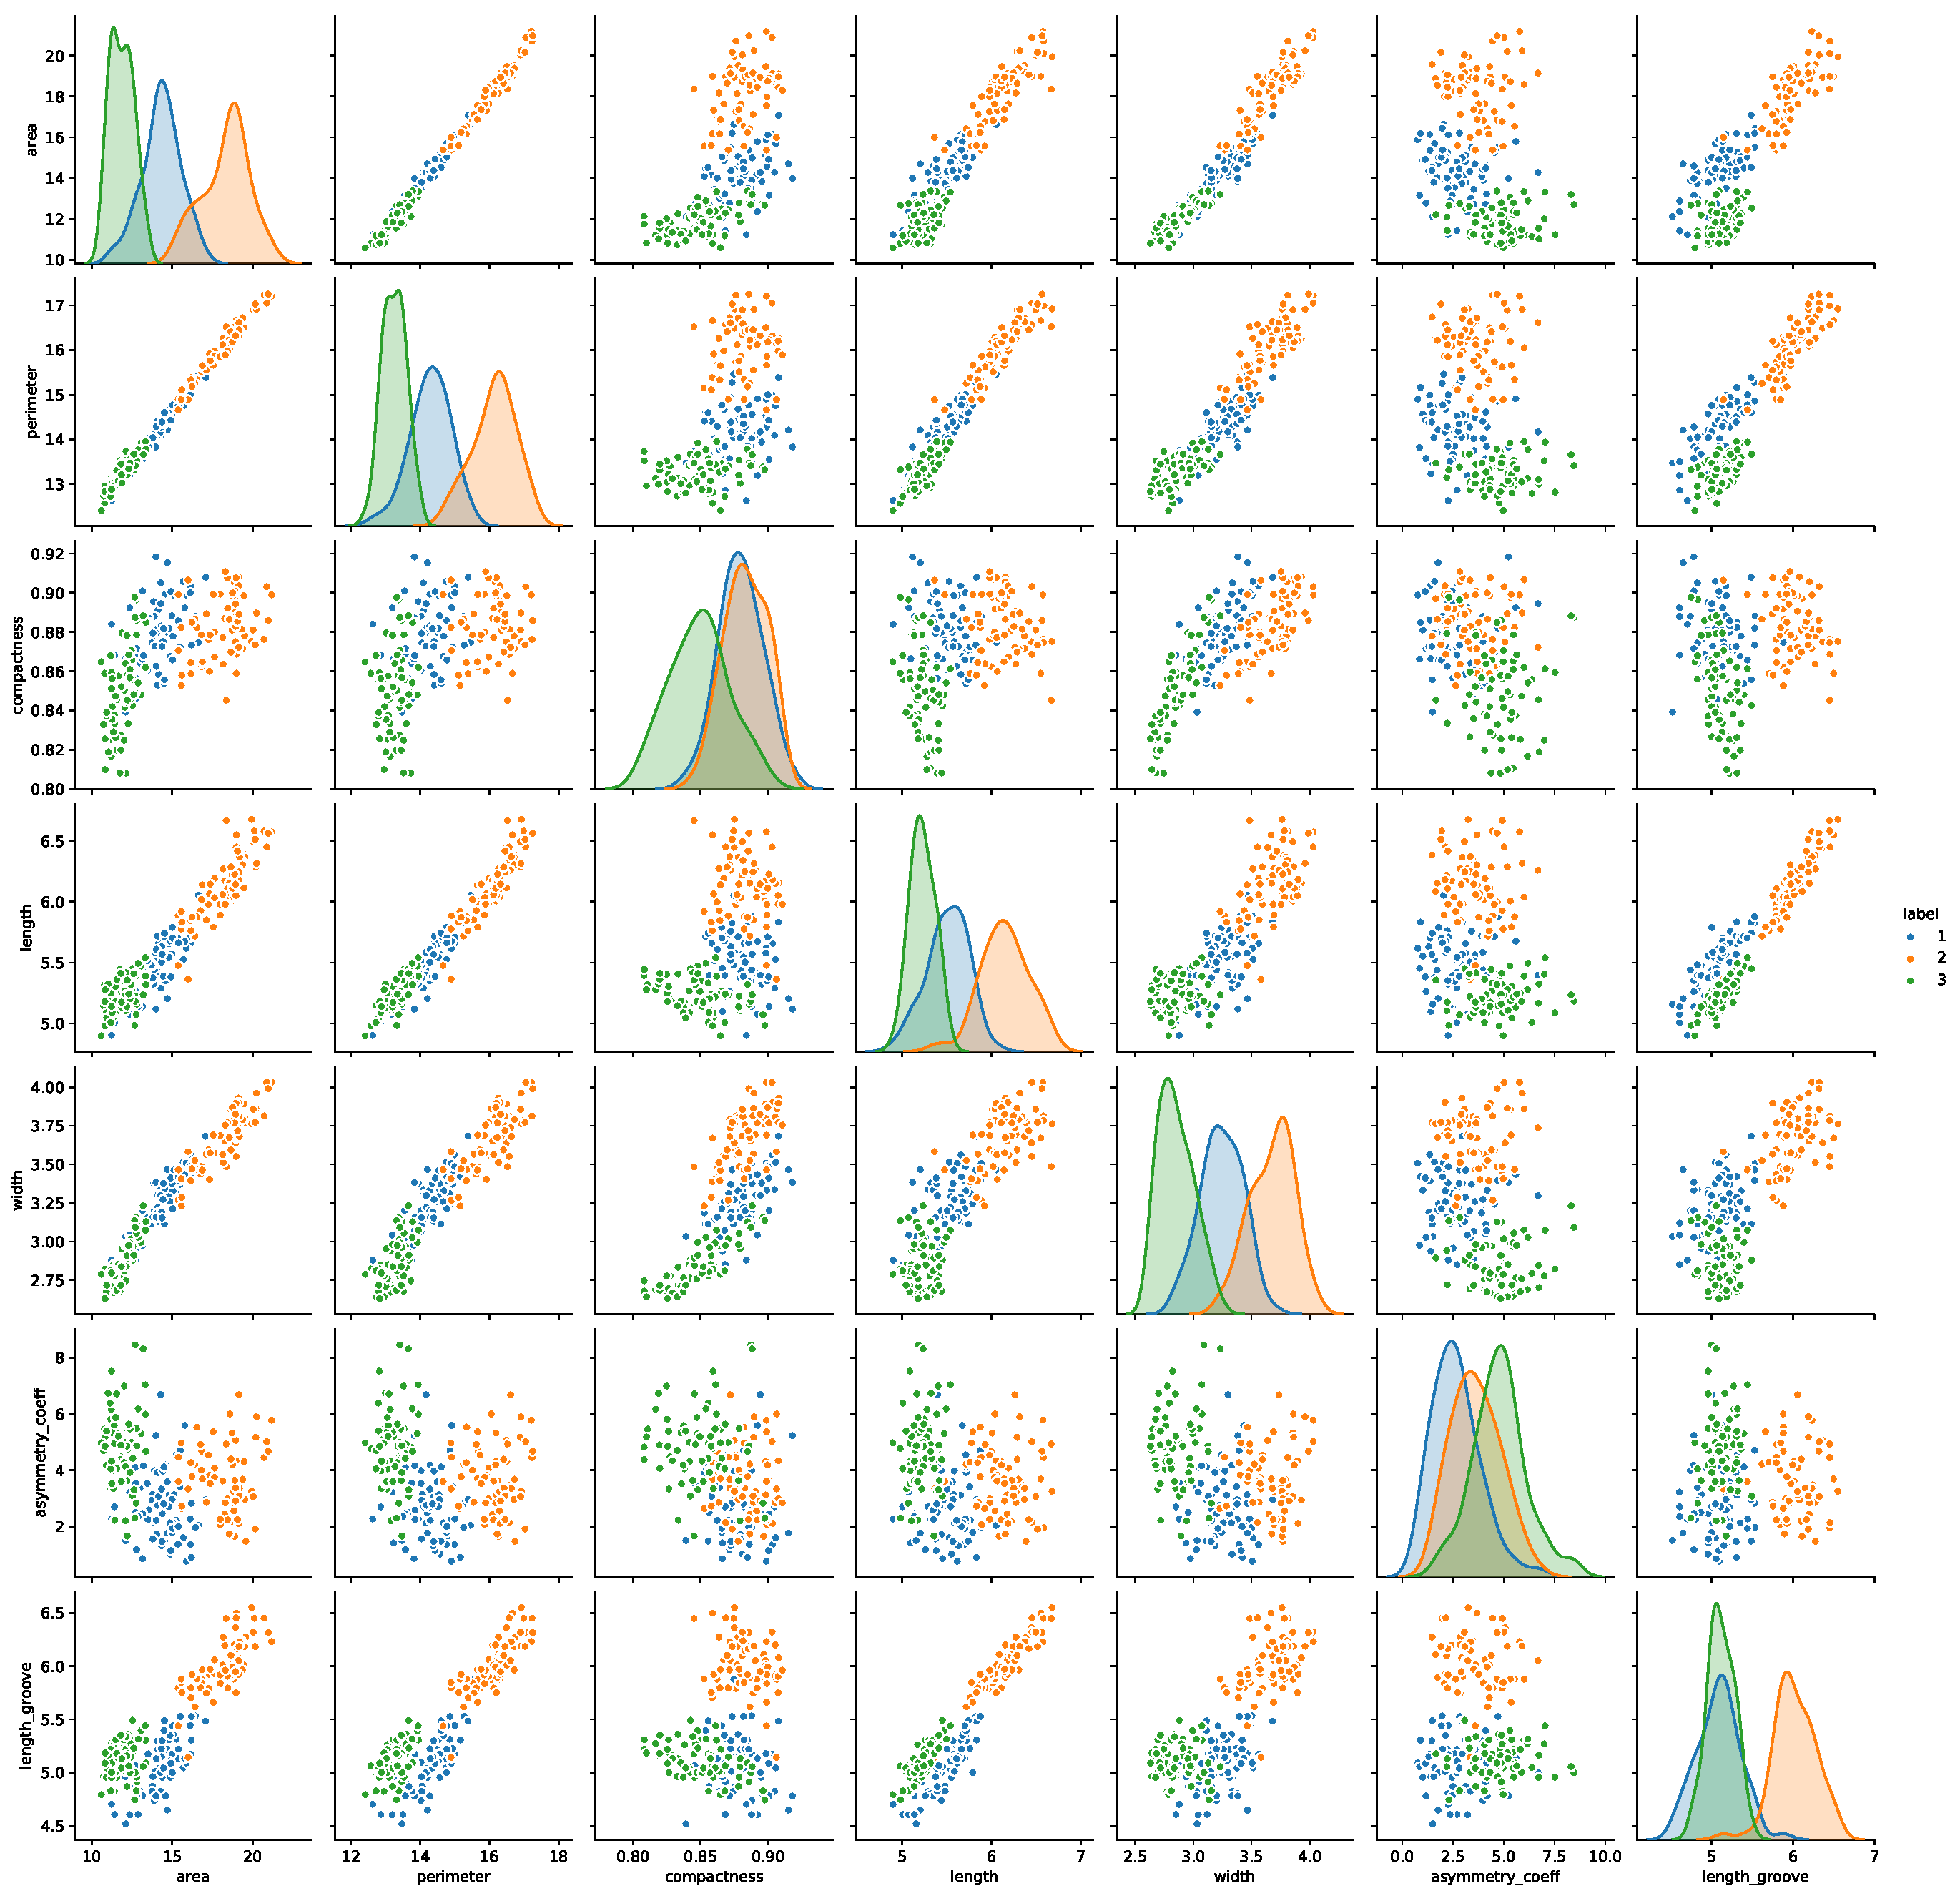
\includepdf[pages=-,scale=.4]{images/seeds_pairplot.pdf}
\begin{center}
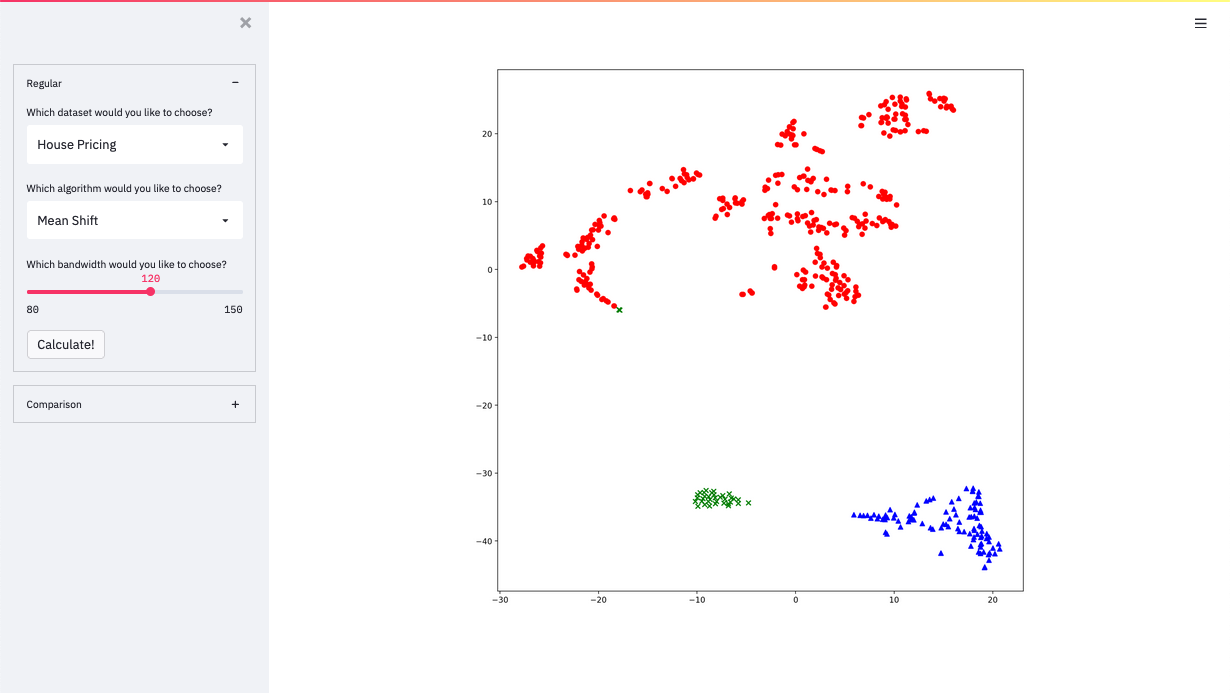
\includegraphics[width=0.9\textwidth]{images/frontend_regular.png}
\caption{Frontend Regular Mean Shift House Pricing Example}
\end{center}
\label{img:frontend_screenshot_regular}
\end{figure}

%In addition to that, we provide an evaluation module which can be used to compare different clustering strategies to each other. 
The \mintinline[bgcolor=code-bg]{python}{Comparison} group contains a singular drop down list which can be used to select the data set of interest. Below this menu, we provide the same type of sliders with the alike functionality as described above, but in this case for all the methods at the same time. Clicking the \mintinline[bgcolor=code-bg]{python}{Compare} button runs all clustering methods with the specified parameters and displays them next to one another in the main panel, similar to the method described above. A table is located below these plots, containing the index values for each index described in section \ref{sec:evaluation_description} (rows) for each clustering method (columns).

\begin{figure}[H]
%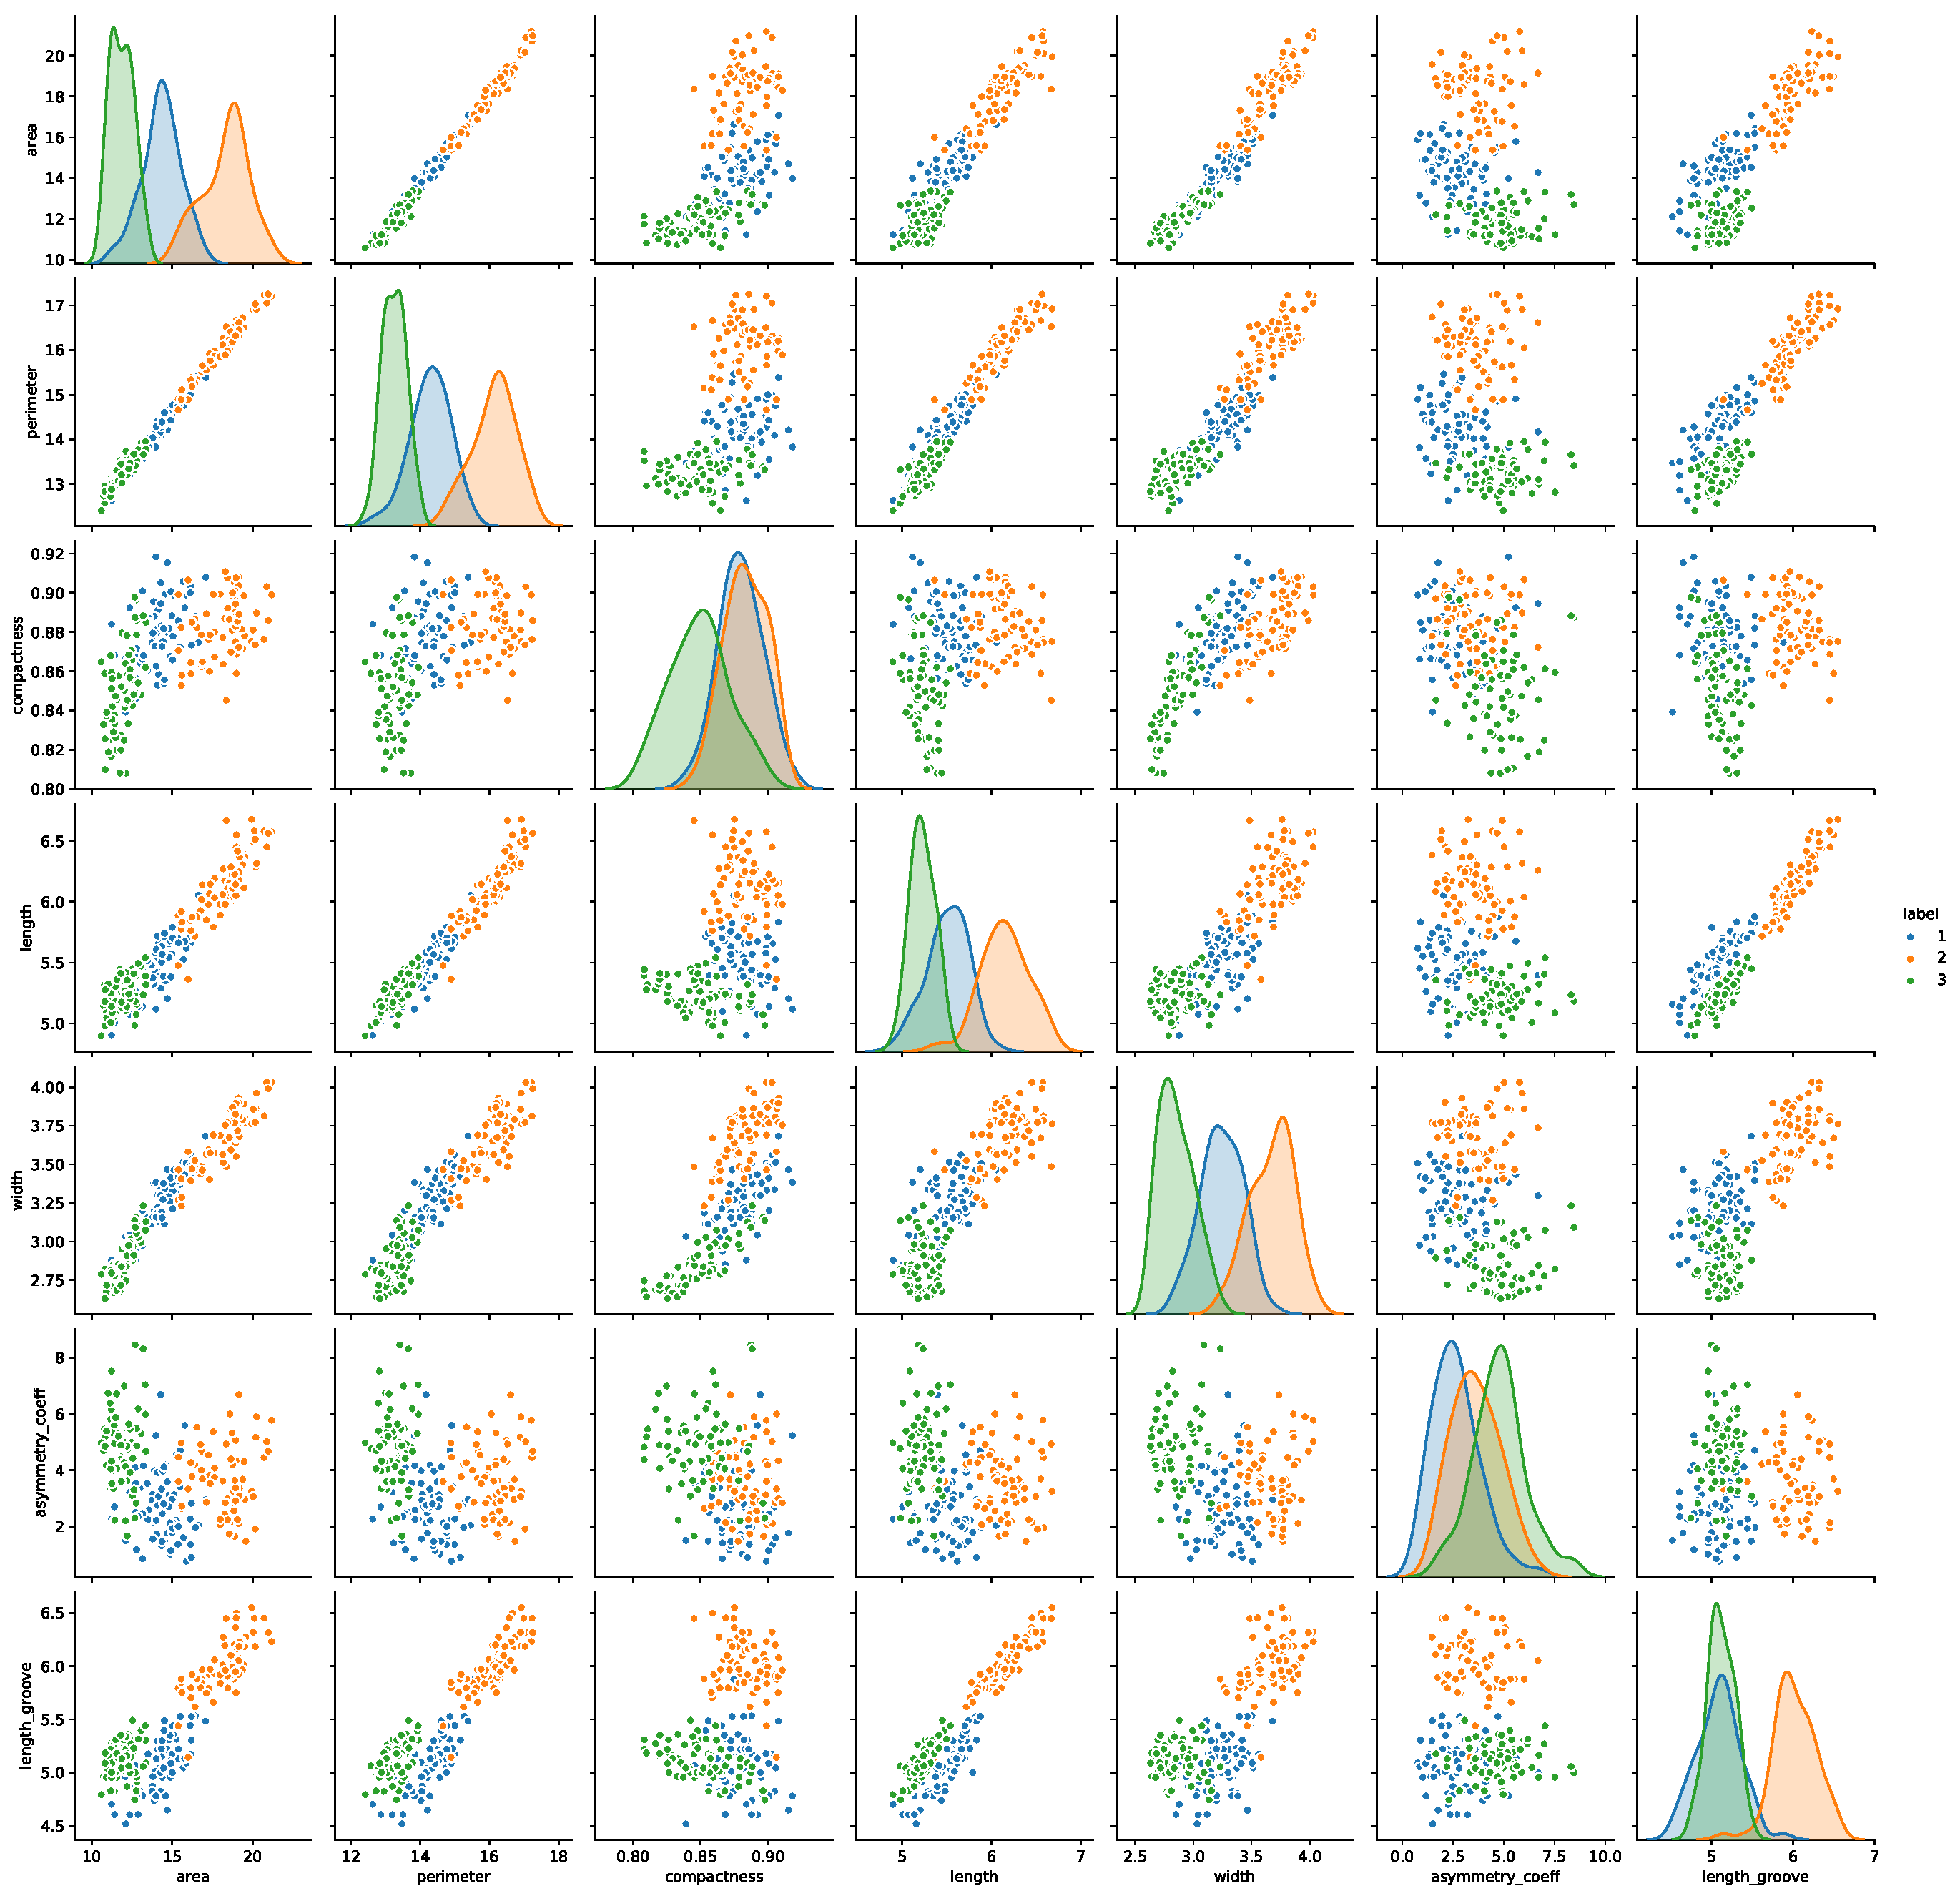
\includepdf[pages=-,scale=.4]{images/seeds_pairplot.pdf}
\begin{center}
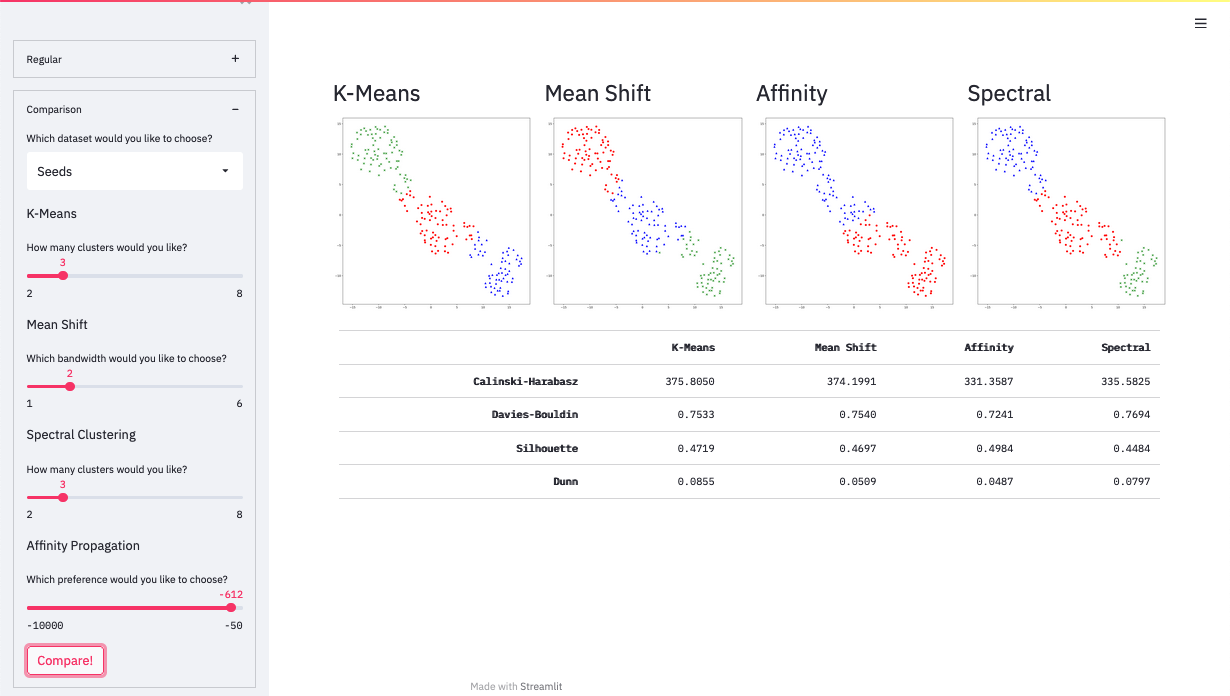
\includegraphics[width=0.9\textwidth]{images/frontend_comparison.png}
\caption{Frontend Comparison Seeds Example}
\end{center}
\label{img:frontend_screenshot_comparison}
\end{figure}

Our code implementation is divided into segments to isolate clustering procedures from projecting the data into 2D and from visualizing the results.

Each of the clustering techniques that can be selected for grouping data points is implemented in a separate file which is named according to the technique. To run one of the clustering algorithms, the data set has to be handed over in form of an $n \times m$ matrix consisting of \textit{n} data points with \textit{m} features. Moreover, a value for the algorithm-specific parameter has to be provided. The \mintinline[bgcolor=code-bg]{python}{returns} parameter can be used to define what output format is expected. We provide the possibility to distinguish between returning the fitted estimator, an $n \times (m+1)$ - matrix consisting of \textit{n} data points with \textit{m} features and a column containing a label for each data point (a task facilitated by \mintinline[bgcolor=code-bg]{python}{numpy} \cite{harris2020array}) or an $n \times 1$ vector, which only includes a label for each data point. These options exist in order to make it possible to return the right format for the task at hand, be it calculations for this work, for evaluation or plotting or inside the frontend itself. Running the clustering in its default mode, each technique returns the $n \times 1$ label vector.
For the K-Means algorithm, the additional parameter \mintinline[bgcolor=code-bg]{python}{state} can be set. This value is used to initialize the random number generator such that always the same results are yielded \cite{sklearn_api}.

In the top level \mintinline[bgcolor=code-bg]{python}{app.py} file, we implement all the functionalities concerning the frontend elements as well as choice of data set and clustering technique. After reading the four different data sets using the \mintinline[bgcolor=code-bg]{python}{read_csv} method provided by pandas \cite{reback2020pandas, mckinney-proc-scipy-2010}, non-numeric values in the data are converted to numeric and we calculate a version of the data sets transformed into 2D and cache it to speed up all following interactions. This is done because transformation into 2D can take long for large data sets. The \mintinline[bgcolor=code-bg]{python}{tsne_transform} function performing this step also takes a state to ensure the resulting plots will always look the same to ease comparability. To transform the data sets into 2D, inside \mintinline[bgcolor=code-bg]{python}{tsne_transform} we make use of the \gls{t-SNE} method provided by \gls{sklearn} \cite{sklearn_api}.

\mintinline[bgcolor=code-bg]{python}{t-SNE} is a method that facilitates displaying high-dimensional data in a 2D or 3D plot while nevertheless preserving local and global structures. This is done converting Euclidean distances between all data points in high dimensions into conditional probabilities such that high probabilities are allocated to similar data points while dissimilar data points are assigned a low probability. Afterwards, the same is done for all the data points projected into lower dimensions. The optimal projection of high-dimensional data points is finally found by minimizing the mismatch between calculated probabilities between points in high and in low dimensions \cite{van2008visualizing}.

As described earlier, we not only provide dropdown lists to enable the choice of a data set as well as a clustering technique, but also adapt the slider widget label according to the required input parameter for the chosen algorithm. We define parameter value ranges along with default values appropriate to the chosen data set. 
To run the clustering procedure, an event handler listens for click events on the \mintinline[bgcolor=code-bg]{python}{Calculate} button. According to the selected clustering algorithm, we call the respective clustering function and hand over the data set as an $n \times m$ - matrix as well as the technique-specific parameter value which was selected with the help of the slider widget.

Largely the same happens when using the \mintinline[bgcolor=code-bg]{python}{Comparison} workflow. The main difference is in the fact that selecting an algorithm is not required because all of them will be run one after the other and plotted next to each other accordingly. The comparison table is then calculated by using the \mintinline[bgcolor=code-bg]{python}{evaluation} module, returning index values and transforming them into an overview.

The plotting as described above is based on \gls{t-SNE} transformation and executed by calling the \mintinline[bgcolor=code-bg]{python}{plot_tsne_2} from the plotting module. The resulting figure comprises scatter plots from the Matplotlib visualization function \mintinline[bgcolor=code-bg]{python}{pyplot} \cite{Hunter:2007} overlayed atop each other for each cluster. This results in one single plot containing all data but each cluster differentiated by color and marker shape making it easy to distinguish between clusters.